Dibuja el sólido cuyo volumen está dado por 
\[
    \int_0^1 \int_0^1 ( 5-x-y ) \,dy\,dx.
\]
\begin{solution}
    La gráfica de la función que se integra corresponde al plano \( z=5-x-y \).
    La base de la figura corresponde al rectángulo \( [ 0,1 ] \times [ 0,1 ] \times \set{0} \).
    El resto de las caras del sólido son los planos que se levantan de los rectángulos.
    \begin{figure}[H]
        \begin{center}
            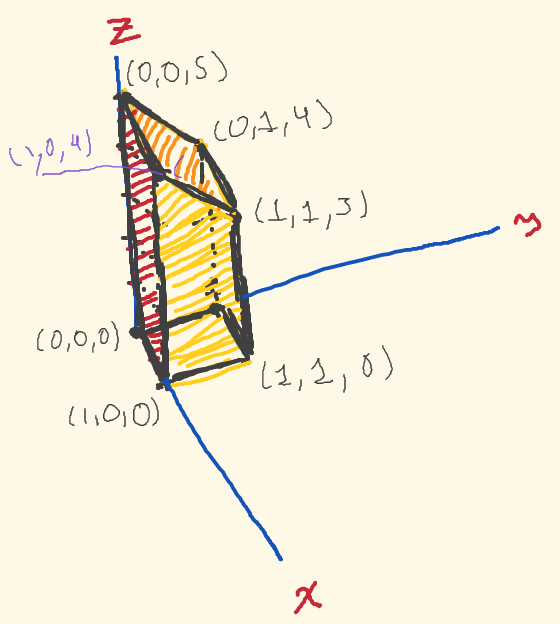
\includegraphics[width=0.3\textwidth]{img/Ej3/ej5.png}
        \end{center}
    \end{figure}
\end{solution}
